
\begin{figure}[htbp]
    \begin{minipage}[t]{0.5\textwidth}
    \centering
    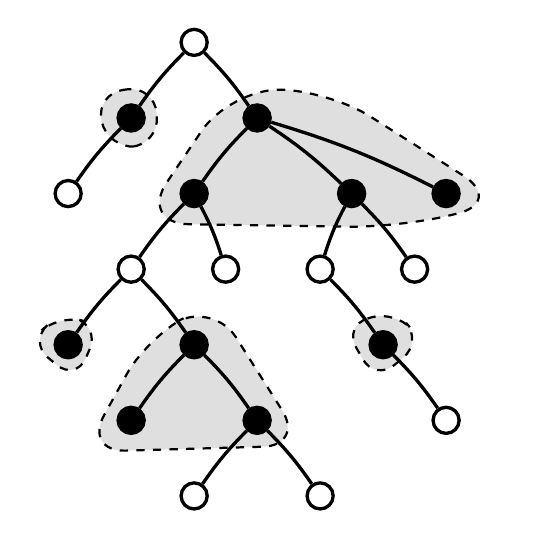
\begin{tikzpicture}[every node/.style={draw, very thick}, every path/.style={very thick}]
    
    \draw[dashed, thick, rounded corners = 10pt, fill= gray!25]
         (-1.25,5.75)  -- (-0.5,5.85)--  (-0.45,5.1) -- (-1.1,5.05) -- cycle;

    \draw[dashed, thick, rounded corners = 18pt, fill= gray!25]
        (0.45,5.8)  -- (1.7,5.8)-- (3.95,4.37) -- (2.6,4.05) -- (-0.7,4.1) -- cycle;
    \draw[dashed, thick, rounded corners = 9pt, fill= gray!25]
        (-2.1,2.6) -- (-1.7,2.95) -- (-1.2,2.8)  -- (-1.5,2.1) -- cycle;
        
    \draw[dashed, thick, rounded corners = 15pt, fill= gray!25]
         (-0.6,2.65) -- (0.25,3.1) -- (1.4,1.28) -- (-1.4,1.2) -- cycle;

    \draw[dashed, thick, rounded corners = 9pt, fill= gray!25]
        (1.9,2.8)  -- (2.55,3)  -- (2.9,2.6) -- (2.3,2.1) -- cycle;
    
    \node[circle, draw, fill=white] (1) at (0,6.4) {};
    
    \node[circle, draw, fill=black] (2) at (-0.8,5.44) {};
    \node[circle, draw, fill=black] (3) at (0.8,5.44) {};

    \node[circle, draw, fill=white] (4) at (-1.6,4.48) {};
    \node[circle, draw, fill=black] (5) at (0,4.48) {};
    \node[circle, draw, fill=black] (6) at (2.0,4.48) {};
    \node[circle, draw, fill=black] (7) at (3.2,4.48) {};
    
    \node[circle, draw, fill=white] (8) at (-0.8,3.52) {};
    \node[circle, draw, fill=white] (9) at (0.4,3.52) {};
    \node[circle, draw, fill=white] (10) at (1.6,3.52) {};
    \node[circle, draw, fill=white] (11) at (2.8,3.52) {};
    
    \node[circle, draw, fill=black] (12) at (-1.6,2.56) {};
    \node[circle, draw, fill=black] (13) at (0,2.56) {};
    \node[circle, draw, fill=black] (14) at (2.4,2.56) {};
    
    \node[circle, draw, fill=black] (15) at (-0.8,1.6) {};
    \node[circle, draw, fill=black] (16) at (0.8,1.6) {};
    \node[circle, draw, fill=white] (17) at (3.2,1.6) {};
    
    \node[circle, draw, fill=white] (18) at (0,0.64) {};
    \node[circle, draw, fill=white] (19) at (1.6,0.64) {};
    
    \draw[bend right=5] (1) to (2);
    \draw[bend left=5] (1) to (3);
    
    \draw[bend right=5] (2) to (4);
    \draw[bend right=5] (3) to (5);
    \draw[bend left=5] (3) to (6);
    \draw[bend left=5] (3) to (7);
    
    \draw[bend right=5] (5) to (8);
    \draw[bend left=5] (5) to (9);
    \draw[bend right=5] (6) to (10);
    \draw[bend left=5] (6) to (11);
    
    \draw[bend right=5] (8) to (12);
    \draw[bend left=5] (8) to (13);
    \draw[bend left=5] (10) to (14);
    
    \draw[bend right=5] (13) to (15);
    \draw[bend left=5] (13) to (16);
    \draw[bend left=5] (14) to (17);
    
    \draw[bend right=5] (16) to (18);
    \draw[bend left=5] (16) to (19);

    \end{tikzpicture}
\end{minipage}
    \begin{minipage}[t]{0.5\textwidth}
    \centering
    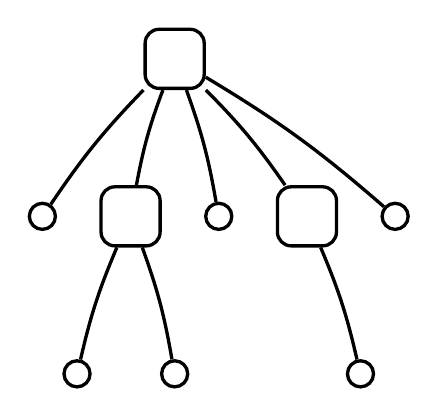
\begin{tikzpicture}[every node/.style={draw,rounded corners=5pt, very thick}, every path/.style={very thick}]
    
    \node[rectangle, minimum size=0.75cm, draw] (1) at (-0.56,10) {};
    
    \node[circle, draw] (2) at (-2.24,8) {};
    \node[rectangle, minimum size=0.75cm, draw] (3) at (-1.12,8) {};
    \node[circle, draw] (4) at (0,8) {};
    \node[rectangle, minimum size=0.75cm, draw] (5) at (1.12,8) {};
    \node[circle, draw] (6) at (2.24,8) {};
    
    \node[circle, draw] (7) at (-1.8,6) {};
    \node[circle, draw] (8) at (-0.56,6) {};
    \node[circle, draw] (9) at (1.8,6) {};
    
    \draw[bend right=5] (1) to (2);
    \draw[bend right=5] (1) to (3);
    \draw[bend left=5] (1) to (4);
    \draw[bend left=5] (1) to (5);
    \draw[bend left=5] (1) to (6);
    
    \draw[bend right=5] (3) to (7);
    \draw[bend left=5] (3) to (8);
    \draw[bend left=5] (5) to (9);

    \end{tikzpicture}
\end{minipage}
    \caption{Example of contracting 5 heavy modules. Black vertices represent heavy vertices, white vertices represent light vertices and square vertices represent vertices which were a parent of at least one heavy module before contraction.}\label{exampleHeavymoduleContraction}
\end{figure}